\chapter{Beispielkapitel}
\section{Beispiele zitieren}

Das ist ein Zitat mit Klammern,
\citep{resnick_distributed_1996}, das ein Zitat ohne Klammern:
\cite{harel_situating_1991}. Hier das selbe Zitat mit einer Seitenangabe und Klammern \citep[S. 23]{resnick_distributed_1996}.

Wird ein Absatz aus einer Quelle sinngemäß übernommen (nicht wörtlich), dann kann nach dem Absatz das entsprechende Zitat in Klammern angeführt werden. \citep[S. 33]{anastopoulou_constructionism_2012}

Wenn ein Zitat im Text angegeben wird, wie z.B. so \cite{beer_rudolf_aspekte_2011}, können die Klammern weggelassen werden.

Der folgende Absatz zeigt ein Blockzitat (wörtlich übernommene Textpassage aus einer Quelle):

\blockcquote[S. 21]{ackermann_piagets_2001}{
Dr. Heinrich Faust ist ein angesehener Wissenschaftler und Akademiker, der trotz seiner wissenschaftlichen Studien und einer guten Bildung seinen Wissensdurst nicht stillen kann. Eines Nachts sitzt er in seinem Studierzimmer und grübelt über den Sinn des Lebens nach, findet jedoch keine Antworten.
Daraufhin wendet er sich der Geisterwelt zu. Er beschwört einen Erdgeist, versucht sich den Geistern gleich zu stellen, was ihm jedoch nicht gelingt. Von Ohnmacht getrieben will er sich das Leben nehmen. Sein Selbstmordversuch wird jedoch von Glockenläuten zum Ostertag und seinen Kindheitserinnerungen gestört.
}

Hier wird ein wörtliches Zitat inline angegeben: \blockcquote{gohlich_lernen:_2007}{Das ist ein kleines direktes Zitat.}, und danach geht es gleich wieder direkt weiter. Ob ein wörtliches Zitat inline oder als eigener Block angezeigt wird, entscheidet Latex auf Basis der Länge.

%So kann man den Author umdefinieren, der für den Seiteninhalt
%verantwortlich ist
\def \currentAuthor {Harald Sohm}

\subsection{Beispiele Abbildungen}
Auf diese Weise kann man zum Beispiel in Latex auf die \cref{fig:ArduExample} verweisen. Die Kennung für den Verweis vergibt
man selbst mit dem "`label"' Kommando bei der Abbildung.

Jede Abbildung muss nicht nur mindestens einen Verweis im Text haben. Es wird außerdem eine Bildunterschrift verlangt. Für diese ist festgesetzt, dass die Abbildungsunterschrift alleine ausreichend sein muss, um zu verstehen, was am Bild zu erkennen ist. 

Der nächste wichtige Punkt sind die Quellenangaben bei Abbildungen. Der Author muss zu jeder Abbildung die notwendigen Rechte haben und idealer Weise gibt man diese bei der Abbildung mit an. In \cref{fig:ArduExample} auf Seite \pageref{fig:ArduExample} sieht man das.

Es ist wichtig zu verstehen, dass Latex die Positionierung von Abbildungen übernimmt. Man definiert die Abbildung über begin-figure dort, wo man die Abbildung in etwa haben  möchte, den Rest übernimmt Latex

\begin{figure}[t]
\centering
%\includegraphics[width=0.7\linewidth]{figures/Arduino_board.png}
\copyrightbox[r]{\includegraphics[width=0.8\linewidth]{figures/Arduino_Example.jpg}}{\textcopyright\
Stefan Stolz (CC BY-SA 3.0)}
\caption[Arduino mit Lichtsensor und Lichterkette]{Hintergrund: Arduino Board;
Vordergrund: eine Lichterreihe und ein Lichtsensor (Fotowiderstand); In diesem
Beispiel wird die Lichterreiche je nach Helligkeit des Umgebungslichtes
gesteuert. Durch leichte Modifikationen kann man damit eine Lichtschranke oder
auch eine Helligkeitssteuerung für das Smartphone simulieren.}
\label{fig:ArduExample}
\end{figure}

\subsubsection{Beispiele Tabellen}

\cref{tbl:shiftReg} ist ein Beispiel für eine aufwändigere Tabelle mit einer
Abbildung und Überschrift.

\begin{table}
     \begin{center}
     \begin{tabularx}{\textwidth}{ cX  } 
      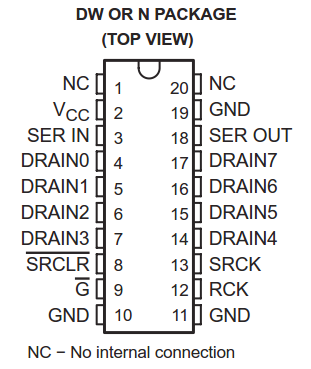
\includegraphics[width=0.3\textwidth]{figures/shift_reg.png}  & 
      {\begin{tabularx}{\cellwidth}{ lX  }      
      $V_{cc}$ & Positive supply voltage\\
      GND & Ground \\
      SER IN & Daten Pin \\
      SRCK & Clock Pin \\
      RCK & Latch Pin \\
      $\overline{SRCLR}$ & Wenn \textbf{shift-register clear} LOW ist, werden die input Register gelöscht\\
      $\overline{G}$ & Wenn \textbf{output enable} HIGH ist, werden die Daten im Output Buffer LOW gehalten
      \end{tabularx}   }
      \end{tabularx}
      \caption{Aufwändige Tabelle mit Abbildung und Caption}
      \label{tbl:shiftReg}
      \end{center}
\end{table}

Tabellen sind in Latex sehr kompliziert zu erzeugen. Alternativ kann man die Tabellen auch in einem anderen Programm gestalten und als Bild wieder einfügen. Dieses Bild kann dann innerhalb von begin-Table verwendet werden.

\section{Beispiele Listen}
Im Folgenden wird eine Liste gezeigt:
\begin{itemize}
  \item Ich weiß, dass viele Geräte des täglichen Lebens durch Computer
  gesteuert werden und kann für mich relevante nennen und nutzen.
  \begin{enumerate}
  	\item Und jetzt eine Numerierung
  	\item Und jetzt eine Numerierung
  \end{enumerate}
  \item Ich kann wichtige Bestandteile eines Computersystems (Eingabe-,
  Ausgabegeräte und Zentraleinheit) benennen, kann ihre Funktionen beschreiben
  und diese bedienen.
\end{itemize}

Und jetzt eine Numerierung:

\begin{enumerate}
	\item Aufzählungspunkt
	\begin{enumerate}
		\item Unteraufzählung
		\item Unteraufzählung
		\begin{itemize}
			\item Und jetzt noch eine Ebene ohne Aufzählung
			\item Und jetzt noch eine Ebene ohne Aufzählung
		\end{itemize}
	\end{enumerate}
	\item Aufzählungspunkt
	\item Aufzählungspunkt
	\item Aufzählungspunkt
	\item Aufzählungspunkt
\end{enumerate}

\section{Beispiel Codesequenz}
In \cref{code:qj} sieht man ein Quick-Sort-Listing in der Programmiersprache JAVA. Das Listings-Paket übernimmt die Formatierung von Codebausteinen und kann in der Präambel nach Belieben auf eine andere Sprache konfiguriert werden.

\def \currentAuthor {Author2}

\subsection{Quicksort in JAVA}
\begin{lstlisting}[language=Java, caption=QuickSort in Java, label=code:qj]
public class QuickSort {
public static void main(String[] args) {
int[] x = { 9, 2, 4, 7, 3, 7, 10 };
System.out.println(Arrays.toString(x));

int low = 0;
int high = x.length - 1;

quickSort(x, low, high);
System.out.println(Arrays.toString(x));
}

public static void quickSort(int[] arr, int low, int high) {
if (arr == null || arr.length == 0)
return;

if (low >= high)
return;

// pick the pivot
int middle = low + (high - low) / 2;
int pivot = arr[middle];

// make left < pivot and right > pivot
int i = low, j = high;
while (i <= j) {
while (arr[i] < pivot) {
i++;
}

while (arr[j] > pivot) {
j--;
}

if (i <= j) {
int temp = arr[i];
arr[i] = arr[j];
arr[j] = temp;
i++;
j--;
}
}

// recursively sort two sub parts
if (low < j)
quickSort(arr, low, j);

if (high > i)
quickSort(arr, i, high);
}
}
\end{lstlisting}

\section{Beispieltext}

\Blindtext